\documentclass[11pt,a4paper]{article}
\usepackage{fullpage, graphicx, url, enumitem, parskip}

\newlist{tip}{itemize}{1}
\setlist[tip,1]{
  leftmargin=\dimexpr1.2cm+\labelsep\relax,
  label={\smash{\raisebox{-0.6\height}{\includegraphics[width=1.5cm]{images/icons/tip.png}}}}
}

\newlist{arrow_red}{itemize}{1}
\setlist[arrow_red,1]{
  leftmargin=\dimexpr0.5cm+\labelsep\relax,
  label={\smash{\raisebox{-0.3\height}{\includegraphics[width=0.5cm]{images/icons/arrow_red.png}}}}
}

\newlist{arrow_yellow}{itemize}{1}
\setlist[arrow_yellow,1]{
  leftmargin=\dimexpr0.5cm+\labelsep\relax,
  label={\smash{\raisebox{-0.3\height}{\includegraphics[width=0.5cm]{images/icons/arrow_yellow.png}}}}
}

\newlist{arrow_blue}{itemize}{1}
\setlist[arrow_blue,1]{
  leftmargin=\dimexpr0.5cm+\labelsep\relax,
  label={\smash{\raisebox{-0.3\height}{\includegraphics[width=0.5cm]{images/icons/arrow_blue.png}}}}
}

\newlist{arrow_green}{itemize}{1}
\setlist[arrow_green,1]{
  leftmargin=\dimexpr0.5cm+\labelsep\relax,
  label={\smash{\raisebox{-0.3\height}{\includegraphics[width=0.5cm]{images/icons/arrow_green.png}}}}
}

\newlist{arrow_pink}{itemize}{1}
\setlist[arrow_pink,1]{
  leftmargin=\dimexpr0.5cm+\labelsep\relax,
  label={\smash{\raisebox{-0.3\height}{\includegraphics[width=0.5cm]{images/icons/arrow_pink.png}}}}
}

\setlength{\parindent}{0em}
\setlength{\parskip}{1em}

\title{\includegraphics[width=12cm]{images/logo.png}\\[1cm]SkySight 101: \\[0.5cm]Eine Einleitung für Segelflieger}
\author{\\Matthew Scutter, Jon Pring, Sophie Curio}
\date{Zuletzt aktualisiert: Oktober 2024}


\begin{document}

\begin{titlepage}
\maketitle
\end{titlepage}

\tableofcontents
\pagebreak

\section{Einleitung}
\subsection{Was ist SkySight}

SkySight ist ein interaktives Wettervorhersageprogramm. Es kombiniert die modernsten Technologien mit einer intuitiven Benutzeroberfläche, um hochauflösende Vorhersagen und leistungsfähige Flugplanungsfunktionen zu ermöglichen.


% \subsubsection{Über uns}


\subsection{Wofür dieses Handbuch gut ist}

Dieses Handbuch gibt eine Übersicht über SkySight. Es dient als Anleitung zu den interaktiven Funktionen im Browser und den mobilen Versionen. Detaillierte Beschreibungen aller Vorhersageparameter sind im Anhang zu finden.



\subsubsection{Updates}

Die Software läuft im Browser, somit ist garantiert, dass SkySight immer auf dem neusten Stand ist. Um sicherzustellen, dass SkySight ohne Probleme läuft, empfiehlt es sich, den Browser auf dem neusten Stand zu halten und regelmäßig zu aktualisieren.

Für LXNav und SeeYou SightSight Nutzer werden regelmäßig Updates innerhalb der regulären Firmware und Software Updates durchgeführt, diese sind zu finden auf \url{http://gliding.lxnav.com} und \url{http://naviter.com}.

\subsubsection{Screenshots}

Dieses Handbuch verwendet Screenshots, um Funktionen zu visualisieren. Diese sind zum Zeitpunkt der Veröffentlichung korrekt, können aber je nach Endgerät, Browser oder Bildschirmauflösung leicht abweichen.

\subsection{SkySight Zugang}
SkySight ist auf 

\url{http://skysight.io}

verfügbar. Dort kann auch ein Abonnement abgeschlossen werden. Mit einem einzigen Abonnement hat man Zugang zu allen Regionen und Funktionen.

Das Passwort kann mit dem \emph{Passwort vergessen} Link auf der Startseite zurückgesetzt werden.

\subsubsection{Kompatibilität}
SkySight funktioniert mit allen modernen Browsern, auf allen Platformen. Wir empfehlen Google Chrome. Unsere Website ist darauf ausgelegt, auf allen Bildschirmgrößen problemlos zu laufen, allerdings wird für einige Funktionen ein größerer Bildschirm benötigt. 

Auf mobilen Endgeräten ist SkySight über den Browser und eine speziell für mobile Geräte ausgelegte Website verfügbar. Es ist uns wichtig, dass SkySight ohne Probleme auf allen Platformen läuft, daher empfinden wir eine App als nicht nötig.

\subsubsection{Naviter SeeYou PC}
SeeYou PC kann mit SkySight verbunden werden, um die Wettervorhersage auf den SeeYou Karten einzublenden. Diese Funktion ist ab SeeYou PC V8.0 verfügbar und kann dazu benutzt werden, den Flug zu planen oder Fluganalysen anzustellen. Weitere Details sind auf \url{http://naviter.com} zu finden.
\subsubsection{Naviter Oudie}
Wetterdaten können heruntergeladen und auf dem Oudie 2, Oudie IGN oder Oudie N dargestellt werden. Eine genauere Anleitung dazu ist unter \ref{subsec:oudie} auf Seite \pageref{subsec:oudie} zu finden.
\subsubsection{LXNav LX80xx/90xx}
SkySight Vorhersagen sind für LXNAV Benutzer, welche die LX80xx und LX90xx Serie benutzen, auf diesen Geräten aufrufbar. Das WiFi Modul muss vorhanden und die Software auf dem neusten Stand sein. Weitere Details und Support für diese Geräte sind auf \url{http://gliding.lxnav.com} verfügbar.
\subsection{SkySight Kontakt}
\subsubsection{Kundenservice}
Die meisten Fragen werden in unserer FAQ oder dieser Anleitung beantworten. Bei Problemen oder Fragen, die hier nicht abgedeckt werden, kann das SkySight Team über das Kontaktformular auf \url{http://skysight.io/contact} kontaktiert werden.
\subsubsection{Rückmeldungen und Anregungen}
Wir versuchen SkySight ständig zu verbessern! Anregungen können an folgende Adresse geschickt werden: 
\begin{flushleft}
\url{skysight@skysight.io}
\end{flushleft}
\section{Erste Schritte}

\subsection{Wähle den Flugzeugtyp}
Wenn SkySight zum ersten Mal aufgerufen wird, muss der Flugzeugtyp ausgewählt werden. Die Optionen sind folgende: Drachen, Ballon, Flugzeug, Gleitschirm und Segelflugzeig. 
\begin{center}
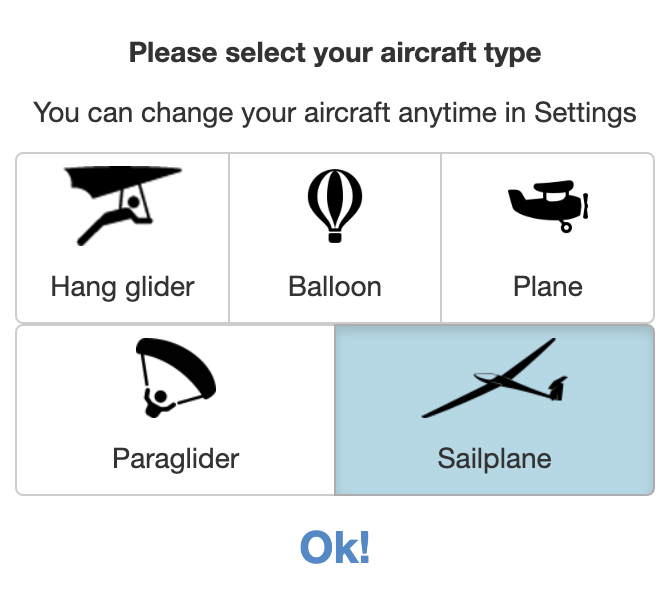
\includegraphics[width=6cm]{images/aircraft_type.png}
\end{center}
Einige Parameter und Fuktionen sind nur für bestimmte Flugzeugtypen vorhanden. Der Flugzeugtyp kann jederzeit geändert werden (siehe \ref{subsec:aircraft_type} auf Seite \pageref{subsec:aircraft_type}). Eine Beschreibung der Flugzeugtyp-spezifischen Parameter und Funktionen sind unter \ref{subsec:specific_features} auf Seite \pageref{subsec:specific_features} zu finden.

\subsection{Benutzeroberfläche}
\subsubsection{Desktop Benutzeroberfläche}
Wenn SkySight aufgerufen wird, erscheint die folgende Benutzeroberfläche:
\begin{center}
\includegraphics[width=12cm]{images/user_interface1.png}
\end{center}
\begin{enumerate}
\item \textbf{Navigationsleiste} -- Hier befindet sich die Navigationsleiste, welche die interaktive Funktionen und Vohersageparameter enthält.
\item \textbf{Datum}  -- Mit \includegraphics[height=9pt]{images/icons/previous.png} und \includegraphics[height=9pt]{images/icons/next.png} kann der gewünschte Tag ausgewählt werden. Die meisten Vorhersageparameter sind bis zu 5 Tage im Voraus verfügbar. Außerdem sind einige zurückliegende Vorhersagen vorhanden.
\item \textbf{Zeit und Zeitzone} -- Mit dem Schieber kann die gewünschte Tageszeit ausgewählt werden. Mit \includegraphics[height=9pt]{images/icons/play.png} kann die Vorhersage animiert werden. Außerdem kann die Zeitzone eingestellt werden.
\item \textbf{Einstellungen} -- In diesem Menü kann die Region geändert werden und die Kontoeinstellungen eingesehen werden. Außerdem ist es möglich, sich hier auszuloggen.
\item \textbf{Kartenansicht} -- Auf der Karte werden die Vorhersageparameter angezeigt. Wie man die Karte navigiert wird in \ref{subsec:mapnav} auf Seite \pageref{subsec:mapnav} erklärte.
\item \textbf{Parameter Beschreibungen} -- Detaillierte Beschreibung des ausgewählten Parameters.
\end{enumerate}
\subsubsection{Mobile Benutzeroberfläche}
Auf mobilen Endgeräten ist die Benutzeroberfläche für kleinere Bildschirme optimiert. Die meisten Funktionen sind auch in der mobilen Ansicht verfügbar, jedoch sind einige erweiterte Funktionen nicht vorhanden.
\begin{center}
\includegraphics[height=8cm]{images/mobile_interface1.png}
\end{center}
\begin{enumerate}
\item \textbf{Navigationsmenü} -- Hiermit kann die Navigationsleiste, welche die interaktive Funktionen und Vohersageparameter enthält, geöffnet und geschlossen werden. Außerdem kann hier der gewünschte Tag ausgewählt werden.
\item \textbf{Zeit und Zeitzone} -- Mit dem Schieber kann die gewünschte Tageszeit ausgewählt werden. Mit \includegraphics[height=9pt]{images/icons/play.png} kann die Vorhersage animiert werden. Die Zeitzone kann geändert werden, indem die `Desktopansicht' im mobilen Browser ausgewählt wird.
\item \textbf{Datum- und Zeitansicht} -- Der ausgewählte Tag und die ausgewählte Zeit wird hier angezeigt.
\item \textbf{Einstellungen} -- In diesem Menü kann die Region geändert werden und die Kontoeinstellungen eingesehen werden.
\item \textbf{Einheiten} -- Hier kann zwischen dem metrischen und dem imperialen Maßsystem gewechselt werden.
\item \textbf{GPS Standort} -- Mit dieser Funktion wird der derzeitige Standort auf der Karte angezeigt. Dafür wird die Ortsbestimmung des Gerätes verwendent (GPS, WiFi or GPRS).
\end{enumerate}

\begin{tip}
\item Mit der \emph{Desktopansicht} können auch alle erweiterten Funktionen in mobilen Browsern benutzt werden.
\end{tip}
\subsection{Kartenansicht} \label{subsec:mapnav}
Auf der Karte werden die Vorhersageparameter angezeigt. Die Karte ist dieselbe auf mobilen Endgeräten und der Desktopversion. Sie wird automatisch aktualisiert, wenn ein neuer Parameter oder eine neue Tageszeit ausgewählt wird.

\subsubsection{Kartenzoom und Navigation}
Die Benutzung der Karte ist für die meisten Nutzer intuitiv. Um die Karte zu bewegen, wird die Karte angeklickt und hin- und hergeschoben.

Die Skala für die ausgewählte Vergrößerung wird in der unteren linken Ecke angezeigt. Am Desktop-Computer kann der Zoom durch scrollen mit der Maus verändert werden. Am Touchscreen wird die Karte mit zwei Fingern vergrößert bzw. verkleinert. Alternativ kann die Vergrößerung mit den + und - Symbolen geändert werden.
\begin{center}
\includegraphics[width=4cm]{images/map_zoom.png}
\end{center}
Wenn `Satellite Map' in der oberen linken Ecke ausgewählt wird, wird eine hochauflösende Luftansicht der Karte angezeigt.

\subsubsection{Vorhersageupdates}
Das Vorhersagemodell läuft mehrmals täglich.
\begin{center}
\includegraphics[width=4cm]{images/last_update.png}
\end{center}
Die Uhrzeit in der unteren linken Ecke der Karte zeigt an, wann die Vorhersage zuletzt aktualisiert wurde. Die Uhrzeit bezieht sich auf den derzeit angezeigten Parameter.

\subsubsection{Farbskala}
Rechts ist die Farbskala zu sehen. Rechts oben wird die Einheit angezeigt. Dort kann zwischen dem metrischen und dem imperialen Maßsystem gewechselt werden. Das Farbschema wird automatisch der Vorhersageregion und der Parameter des Tages angepasst.

\subsubsection{Farbtransparenz für farbenblinde Benutzer}\label{subsec:colorblind}
\begin{center}
\includegraphics[width=6cm]{images/map_color1.png}
\includegraphics[width=6cm]{images/map_color2.png}
\end{center}

Für farbenblinde Benutzer haben wir die Option eingebaut, die Transparenz der Vorhersagekarten zu ändern. Damit werden die Farbtöne kräftiger und mit einem stärkeren Kontrast dargestellt. Um die Transparenz zu verändern, kann der Schieber, welcher sich unten in der Mitte der Karte befindet verschoben werden.

\subsubsection{Genauer Vorhersagewert}
\begin{center}
\includegraphics[width=4cm]{images/exact_value.png}
\end{center}

Wenn ein Vorhersageparameter ausgewählt wurde, kann durch Rechtsklick auf die Karte der genaue Wert angezeigt werden. Zusammen mit der farbkodierten Karte kann dies benutzt werden, um sich eine detaillierte Übersicht über die Vorhersage zu verschaffen.

In der mobilen Version erscheint der genauer Vorhersagewert, wenn man zwei Sekunden lang auf den gewünschten Punkt drückt.

\begin{tip}
\item Der Punkt wird auf der Karte angezeigt, bis er durch Anklicken von x geschlossen wird. Um zu sehen, wie sich der Tag entwickelt, kann die Tageszeit geändert werden.
\end{tip}

\subsubsection{Luftraum Ansicht}
Mit dem \includegraphics[height=15pt]{images/icons/airspace.png} Luftraum Schaltfläche kann der Luftraum auf der Karte angezeigt werden. Dieser ist nur indikativ, für Navigationszwecke sollten Piloten immer aktuelle ICAO Karten verwenden und NOTAMs überprüfen.
\begin{center}
\includegraphics[width=8cm]{images/airspace.png}
\end{center}

\subsubsection{Satellitenansicht} \label{subsec:satview}
Aktuelle Satellitenbilder können mit der \includegraphics[height=12pt]{images/icons/sat.png} Satellitenbild Schaltfläche angezeigt werden. Diese sind für den jetzigen und zurückliegende Zeitpunkte verfügbar.

\begin{tip}
\item Die Vorhersage kann mit dem aktuellen Satellitenbild verglichen werden, indem der `Bedeckungsgrad' ausgewählt wird. Das ermöglicht den direkten Vergleich zwischen Vorhersage und der tatsächlichen Situation.\end{tip}

% \subsubsection{Webcams} \label{subsec:webcams}
% Mit der 
\includegraphics[height=15pt]{images/icons/webcam.png} Webcam Funktion werden aktuelle Webcam Aufnahmen auf der Karte angezeigt. Wenn man mit der Maus über ein Bild fährt, wird es automatisch vergrößert. Diese Funktion kann dazu verwendet werden, sich einen Überblick über die momentane Wettersituation im Aufgabenbereich zu verschaffen.

% \begin{center}
% 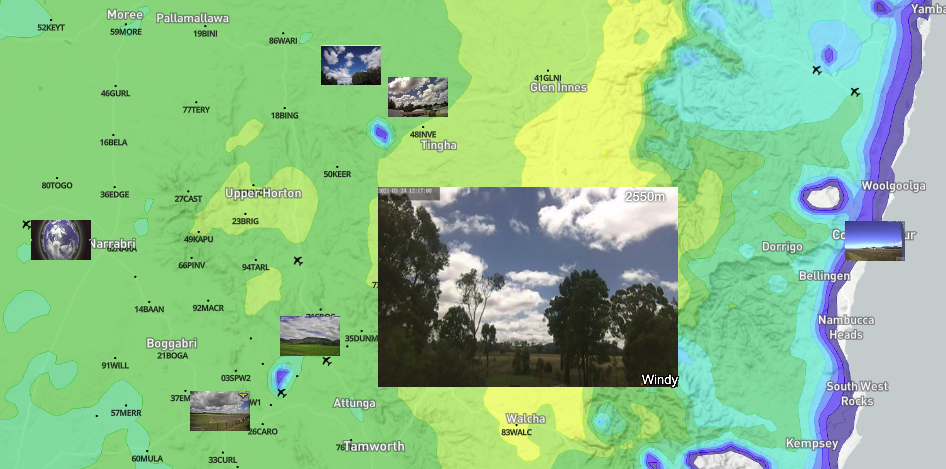
\includegraphics[width=12cm]{images/webcam.png}
% \end{center}

\subsubsection{Cu Übersicht}\label{subsec:cu_overview}
Die Cu Übersicht visualisiert die Verteilung der Cumuluswolken, der Überentwicklung und der Wolkenbedeckung. Eine höhere Dichte von Punkten zeigt zunehmend dickere und überentwickelte Cumuluswolken an. Die graue Wolkenbedeckung zeigt die mittlere bis hohe Wolkenbedeckung an. Die weiche Hintergrundfarbe zeigt die Höhe der trockenen Thermik an. 
\begin{center}
\includegraphics[width=15cm]{images/cu_overview_german.png}
\end{center}

\subsubsection{Signifikantes Wetter}
Die Signifikantes Wetter Karte gibt einen Überblick über das Wetter in dem Aufgabenbereich. Durch verschiedene Symbole werden Wetterereignisse wie Wolken, Regen, Wind oder Stürme angezeigt. 
\begin{itemize}
  \item 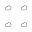
\includegraphics[height=15pt]{images/icons/cu-1.png} Vereinzelte Cumuluswolken
  \item 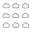
\includegraphics[height=15pt]{images/icons/cu-2.png} Cumuluswolken
  \item 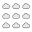
\includegraphics[height=15pt]{images/icons/cu-od-3.png} Dichte Cumuluswolken
  \item 
\includegraphics[height=15pt]{images/icons/cu-od-4.png} Überentwicklung
  \item 
\includegraphics[height=15pt]{images/icons/cu-rain-7.png} Regen
  \item 
\includegraphics[height=15pt]{images/icons/cu-storm-6.png} Potenzielle Sturmgefahr
\end{itemize}

\subsubsection{Es wird nichts angezeigt?}
Wenn auf der Karte nichts angezeigt wird, kann das mehrere Gründe haben.
\begin{itemize}
\item Das ausgewählte Datum liegt außerhalb des Vorhersagebereiches. 
\item Eine andere Region ist aktiv. In den Einstellungen wird die ausgewählte Region angezeigt und kann geändert werden.
\item Der ausgewählte Parameter ist für den Vorhersagezeitraum nicht verfügbar. Einige Parameter sind nur für die nächsten paar Tage verfügbar, da sie sonst zu ungenau werden oder rechenintensiv sind.
\item Die Kartentransparenz liegt bei 0. In dem \ref{subsec:colorblind} Abschnitt auf Seite \pageref{subsec:colorblind} wird erklärt, wie die Transparenz eingestellt wird.
\item Die Satellitenbildansicht ist an. In dem \ref {subsec:satview} Abschnitt auf Seite \pageref{subsec:satview} wird erklärt, wie diese abgestellt wird.
\item Manchmal sind die Vorhersagedaten sehr groß, dadurch kann es bei langsamen Internetverbindungen zu Verzögerungen kommen.
\end{itemize}

\section{Interaktive Funktionen}
SkySight enthält einige interaktive Funktionen, die die Vorhersage- und Routenplanung einfacher machen. In diesem Abschnitt werden die Grundlagen dieser Funktionen erklärt.
\subsection{Temp}
Diese Funktion zeigt ein Vertikalprofil für jeden möglichen Punkt auf der Karte zu jeder beliebigen Uhrzeit an.
\begin{center}
\includegraphics[width=12cm]{images/skew-t.png}
\end{center}
\begin{arrow_red}
\item \textbf{Temperaturkurve} Die vorhergesagte Temperatur der Umgebungsluft in Abhängigkeit von der Höhe.
\end{arrow_red}
\begin{arrow_green}
\item \textbf{Taupunktkurve} Die vorhergesagte Temperatur des Taupunkts in Abhängigkeit von der Höhe.
\end{arrow_green}
\begin{arrow_blue}
\item \textbf{Windstärke} Die vorhergesagte Windstärke in Abhängigkeit von der Höhe. Windfieder werden auch angezeigt.
\end{arrow_blue}
\begin{arrow_pink}
\item \textbf{Virtuelles Luftpaket} Ein simuliertes Paket heißer Luft, welches durch die Grenzschicht steigt. Diese Funktion wird dazu verwendet, eventuelle Gewitter vorherzusagen.
\end{arrow_pink}
Wie man die Temp Funktion verwendet:
\begin{enumerate}
\item Zuerst muss die  \includegraphics[height=15pt]{images/icons/skew-t.png} Funktion in der Menüleiste ausgewählt werden.
\item Es kann auf jeden beliebigen Punkt auf der Karte geklickt werden, um das gewünschte Vertikalprofil/Temp aufzurufen.
\item Die Zeit kann mit dem Schieber eingestellt werden, dadurch kann man sehen, wie sich die Vorhersage über den Tag entwickelt. 
\item Die Temperatur und Wind für jede beliebige Höhe wird angezeigt, wenn man mit der Maus über die Graphik fährt.
\item Mit \includegraphics[height=11pt]{images/icons/exit.png} in der rechten oberen Ecke des Bildschirms wird die Funktion geschlossen.
\end{enumerate}
\begin{tip}
\item Das Vertikalprofil kann nicht nur dabei helfen, die Vorhersage zu verstehen, es zeigt auch die Luftfeuchtigkeit in höheren Luftmassen an und hilft dabei, die Überentwicklung und Wolkenbedeckung zu verstehen und vorherzusagen.
\end{tip}
\subsection{Lokale Vorhersagen}
Die `Lokale Vorhersagen' Funktion ermöglicht es, den Verlauf des Wetters über den Tag einfach und schnell zusammenzufassen. Wolkenbedeckung, thermische Aktivität und Temperatur werden visualisiert und als Werte dargestellt.

Um die lokale Vorhersage zu benutzen:
\begin{enumerate}
\item Wählen Sie zunächst die \includegraphics[height=15pt]{images/icons/point_forecast.png} `Lokale Vorhersage' Funktion in der Menüleiste aus, die Funktion ist dann blau hinterlegt.
\item Klicken Sie nun auf jeden beliebigen Punkt auf der Karte, um die gewünschte lokale Vorhersage aufzurufen.
\item Ggf. müssen Sie nach unten scrollen, um alle Parameter zu sehen.
\item Den genauen Ort der lokalen Vorhersage können Sie ändern, indem Sie den blauen Positionsmarker verschieben. Auf mobilen Endgeräten wird die Karte nicht angezeigt, stattdessen müssen Sie die lokale Vorhersage schließen und einen neuen Punkt auswählen.
\item Klicken Sie auf \includegraphics[height=11pt]{images/icons/exit.png}, um die Vorhersage zu schließen.
\end{enumerate}
\begin{center}
\includegraphics[width=12cm]{images/point_forecast.png}
\end{center}
Die Bewölkung wird in der obersten Reihe in Form eines Farbgradienten angezeigt. Blau bedeutet klares Wetter, weiß bedeutet dünne Wolken und dunklere Grautöne weisen auf eine dickere Wolkendecke hin.

Die Höhe der Cumuluswolken wird als ein grau hinterlegter Bereich über der Kondensationslinie angezeigt. Wenn kein grauer Bereich zu sehen ist, weist es auf blaue Thermik hin.

\subsection{Punkt-Winddiagramm}
Das Winddiagramm zeigt die Entwicklung des Temperaturgefälles, der Temperatur, der relativen Feuchtigkeit und des Windes über den Tag in Abhängigkeit von der Höhe an. Mit dieser Funktion können Inversionen, Feuchtigkeitsschichten und Windgradienten visualisiert werden.
\begin{center}
\begin{minipage}{\textwidth}
\centering
\textbf{Übersicht}

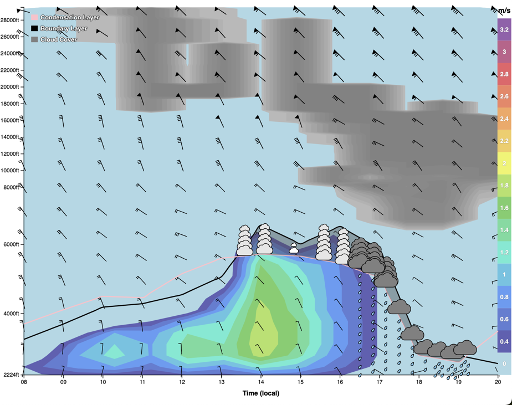
\includegraphics[width=10cm]{images/windgram_overview.png}
\end{minipage}

\begin{minipage}{0.45\textwidth}
\centering
\textbf{Temperaturgefälle}

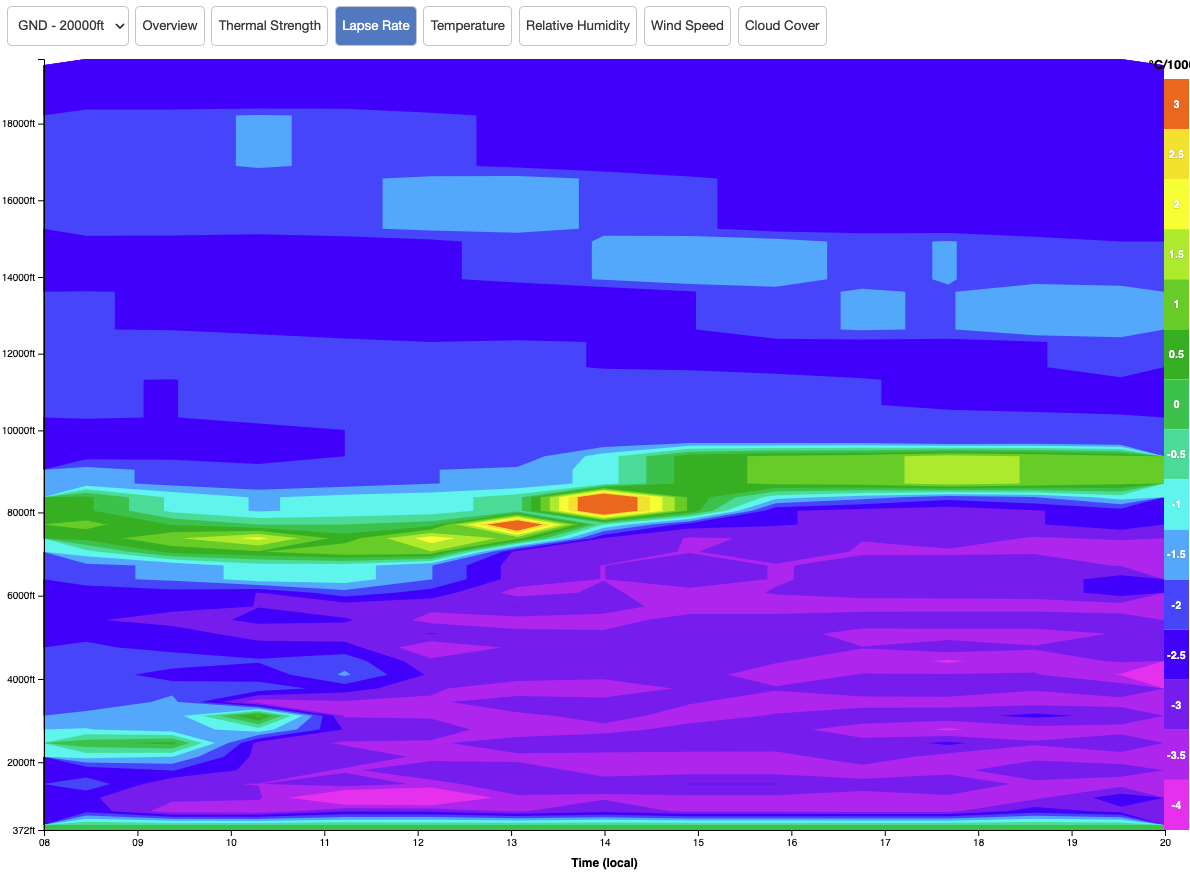
\includegraphics[width=6cm]{images/windgram_lapse.png}
\end{minipage}
\hfill
\begin{minipage}{0.45\textwidth}
\centering
\textbf{Wind}

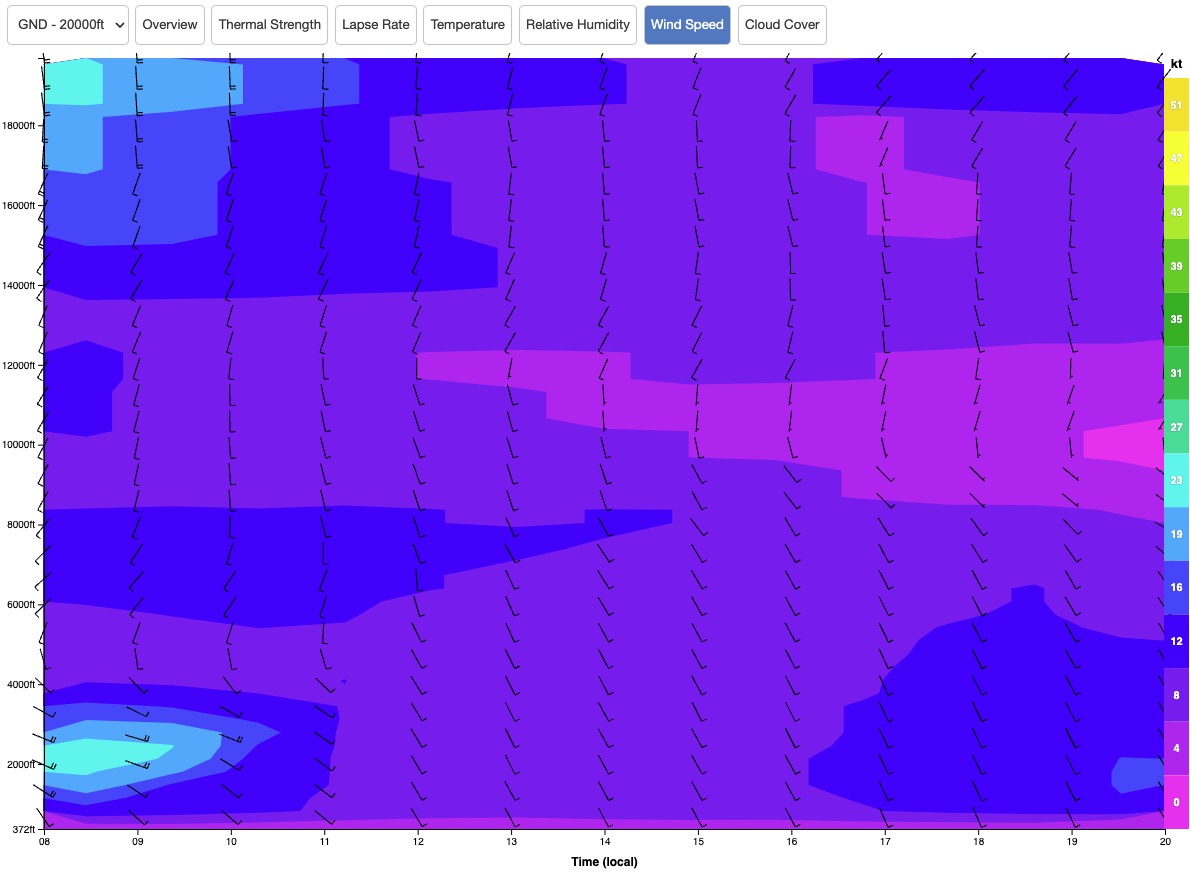
\includegraphics[width=6cm]{images/windgram_wind.png}
\end{minipage}
\end{center}

Wie man das Winddiagramm verwendet: 
\begin{enumerate}
\item Wählen Sie die \includegraphics[height=15pt]{images/icons/windgram.png} `Winddiagramm' Funktion in der Menüleiste aus, die Funktion ist dann blau hinterlegt.
\item Klicken Sie nun auf jeden beliebigen Punkt auf der Karte, um das gewünschte Winddiagramm aufzurufen.
\item In dem Aufklappmenü können Sie den Parameter ändern. Es stehen insgesamt sechs Parameter zur Verfügung: Übersicht, Thermikstärke, Temperaturgefälle, Temperatur, relative Feuchtigkeit, Wind und Bedeckungsgrad.
\item Um Windfieder an- oder abzuschalten, klicken Sie die Box neben dem Aufklappmenü an.
\item Um das Winddiagramm zu schließen, klicken Sie auf \includegraphics[height=11pt]{images/icons/exit.png}.
\end{enumerate}

\subsection{Routenvorhersage}\label{subsec:routeforecast}
Mit der Routenvorhersage wird die erwartete Streckengeschwindigkeit berechnet. Außerdem wird eine Übersicht über die Vorhersagen auf der geplanten Strecke angezeigt. Mit dieser Funktion lassen sich Flüge, inklusive Wettbewerbsflüge planen. Indem die Wegpunkte verschoben werden, lässt sich einfach die schnellst mögliche Aufgabe finden.
\begin{center}
\includegraphics[width=12cm]{images/route.png}
\end{center}

Wie man die Routen Vorhersage verwendet:
\begin{enumerate}
\item Wählen Sie die \includegraphics[height=15pt]{images/icons/route.png} `Routenvorhersage' Funktion in der Menüleiste aus, die Funktion ist dann blau hinterlegt.
\item Klicken Sie auf die Karte, um den gewünschten Startpunkt auszuwählen. Sie können entweder eine eigene Strecke zeichnen, oder eine der vorgeschlagenen Aufgaben auswählen (grün = kurze Aufgabe, passend für Vereinspiloten am Nachmittag, gelb = mittelschwere Strecke, mit früherem Start und späterer Landung, rot = eine Aufgabe, für die vermutlich der ganze Tag benötigt wird. Passend für erfahrene Piloten, die in schwierigen Bedingungen fliegen möchten.) 
\item Mit jedem weiteren Klick entsteht ein neuer Wendepunkt. Das kann so oft wie nötig wiederholt werden. 
\item Die Route wird bestätigt, indem Sie auf Startpunkt klicken oder `ESC' drücken. Die optimale Startzeit, eine Übersicht über die Vorhersage, die optimale Strecke (schwarze Linie) und die Länge der Strecke wird dann angezeigt.
\item SkySight wählt automatisch das beste Zeitfenster aus, jedoch können Sie dieses auch manuell einstellen, indem Sie die rote Start- und Endzeit verschoben werden. 
\item Die Wendepunkte der Route können Sie jederzeit modifizieren, indem Sie diese anklicken und an die gewünschte Stelle ziehen. Außerdem können neue Wendepunkte hinzugefügt werden - wenn Sie den kleinen roten Punkt zwischen zwei Wendepunkten bewegen, wird dieser zu einem neuen Wendepunkt. 
\item Wenn Sie mit der Maus über die Routenübersicht fahren, welche sich überhalb der Karte befinde, wird auf der Karte die ungefähre Lage zu der entsprechenden Tageszeit angezeigt. Die Routenübersicht zeigt entweder die direkte oder die optimierte Route an - je nachdem, ob `Point-to-Pont' (direkte Route) oder `Optimized' (optimierte Route) ausgewählt wurde. 
\item Die Route wird in der Seitenleiste gespeichert und ist auf allen mit dem Account verbundenen Geräten abrufbar. Mit 
\includegraphics[height=15pt]{images/icons/download.png} lässt sich die Aufgabe herunterladen und mit 
\includegraphics[height=15pt]{images/icons/x.png} aus der Seitenleiste entfernen. 
\item Die Routenvorhersage wird geschlossen, indem Sie auf das \includegraphics[height=15pt]{images/icons/route.png} Routenvorhersage Icon klicken.
\end{enumerate}
Die Routenvorhersage funktioniert am besten bei Aufgaben, die in der Thermik geflogen werden. Die grau hinterlegte Fläche zeigt die Tiefe der Cumuluswolken an. Die Streckengeschwindigkeiten, welche rechts neben der Übersicht unter `Optimale Startzeit' angezeigt werden gelten für einen 18m Ventus 2 @ 45kg/m\(^2\) mit optimaler McCready Einstellung.
\begin{tip}
\item Im Abschnitt \ref{subsec:taskplan} auf Seite \pageref{subsec:taskplan} sind weitere Tips zu finden, wie man die Routenvorhersagefunktion für Routenplanung benutzen kann.
\end{tip}

\subsection{Wellen Querschnitt}
Mit dem Wellenquerschnitt können die Eigenschaften der Welle über eine bestimmte Strecke visualisiert werden. Diese Funktion ist nur in der Desktopversion verfügbar.
\begin{center}
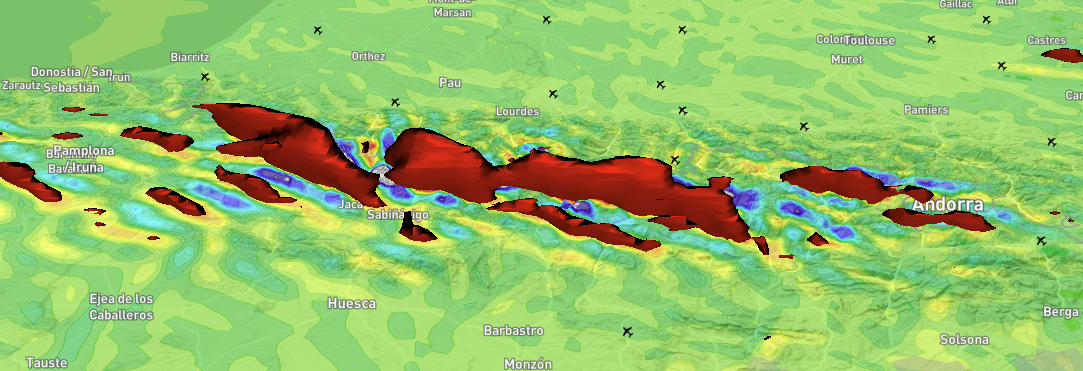
\includegraphics[width=12cm]{images/3dwave.png}
\end{center}

Wie man die Wellen Querschnitt Funktion verwendet:
\begin{enumerate}
\item Wählen Sie die \includegraphics[height=15pt]{images/icons/wave.png} Wellen Querschnitt Funktion in der Menüleiste unter `Welle' aus.
\item Klicken Sie auf die Karte, um den gewünschten Startpunkt auszuwählen.
\item Wählen Sie den Endpunkt mit einem zweiten Klick aus. Dann erscheint der Querschnitt.
\item Auf großen Bildschirmen erscheint die Karte neben dem Querschnitt. Die Start- und Endpunkte können Sie beliebig verschieben. Wenn Sie mit der Maus über den Querschnitt fahren, wird die vertikale Geschwindigkeit und Position auf der Karte angezeigt.
\item Das Bild ist eine Momentaufnahme zu einem bestimmten Zeitpunkt. Um die Entwicklung der Welle über den Tag zu betrachten, können Sie die gewünschte Zeit mit dem Schieber in der oberen Leiste einstellen.
\item Schließen Sie den Wellen Querschnitt, indem Sie auf das \includegraphics[height=15pt]{images/icons/exit.png} Routenvorhersage Icon klicken.
\end{enumerate}

\subsection{3D Welle}
Mit der 3D Wellenfunktion lässt sich die Welle in drei Dimensionen darstellen. Dies erlaubt die Visualisierung der vertikalen und horizontalen Ausdehnung des Wellensystems. Es kann dabei helfen, zu verstehen, wie die Welle sich in der Höhe entwickelt und wo sie besonders hoch ist.
\begin{enumerate}
\item Um die 3D Welle anzuzeigen, klicken Sie auf \includegraphics[height=15pt]{images/icons/wave.png}. 
\item Sie können rein- und rauszoomen, die Karte verschieben und das Wellensystem aus verschieden Richtungen betrachten.
\item Um die 3D Funktion zu schließen, klicken Sie auf \includegraphics[height=11pt]{images/icons/exit.png}.
\end{enumerate}

\section{Erweiterte Funktionen}
\subsection{Anzeigen der Wegpunkte}
Um die Streckenplanung zu unterstützen, können Wegpunkte hochgeladen werden. Diese werden dann als Punkte auf der Karte angezeigt. Ggf. muss die Zoomeinstellung geändert werden um den vollen Namen der Wegpunkte zu sehen.
\begin{center}
\includegraphics[width=12cm]{images/waypoint.png}
\end{center}
Mit der \includegraphics[height=15pt]{images/icons/waypoint.png} Funktion werden Wegpunkte hochgeladen. Es öffnet sich ein Menü, in dem die gewünschte Wegpunktedatei ausgewählt wird. Bei der Datei muss es sich um eine SeeYou cup Datei handeln.

Es kann nur eine Datei auf einmal hochgeladen werden und die Wegpunkte werden nur auf dem Gerät angezeigt, auf dem sie hochgeladen wurden.

Wenn eine Wegpunktdatei vorhanden ist, benutzt die Routenvorhersage (siehe \ref{subsec:routeforecast} auf Seite \pageref{subsec:routeforecast}) automatisch diese Wegpunkte, wenn eine neue Aufgabe ausgewählt oder eingezeichnet wird. 

\subsection{Hochladen von IGC Dateien zur Fluganalyse}
SkySight kann dazu verwendet werden, den Flug im Nachhinein zu analysieren. Das kann von Nutzen sein, um Wetterbeobachtungen, welche im Flug gemacht wurden zu bestätigen. Außerdem kann es dabei helfen, die Entwicklung und Interpretation der SkySight Vorhersage zu verstehen.

\begin{center}
\includegraphics[width=8cm]{images/igc_upload.png}
\end{center}

Mit der \includegraphics[height=15pt]{images/icons/igc.png} IGC Upload Funktion werden IGC Dateien hochgeladen. Der Flug wird dann auf der Karte angezeigt und ermöglicht den direkten Vergleich zwischen den Vorhersage Parametern und der geflogenen Strecke.

Um zum richtigen Tag zu gelangen, muss der Tag manuell ausgewählt werden. Momentan ist es nicht möglich, den Flug abzuspielen, es wird lediglich die geflogene Strecke auf den SkySight Karten angezeigt.

\subsection{Experimentelle Funktionen}
SkySight wird ständig weiterentwickelt und neue Funktionen werden regelmäßig hinzugefügt.

\subsection{Flugzeugtype-spezifische Funktionen}\label{subsec:specific_features}
Einige Parameter und Funktionen, wie die PFD, XC Speed und Routenvorhersage berücksichtigen den Flugzeugtyp. Bestimmte Parameter sind nur zu sehen, wenn ein bestimmter Flugzeugtyp ausgewählt wurde.
\subsubsection{Gleitschirm Startplätze}
Die Startplätze für Gleitschirme sind auf der Karte als Symbol (\includegraphics[height=12pt]{images/icons/paraglider_launch.png}) dargestellt. Die Füllfarbe zeigt an, ob ein bestimmter Standort für einen Start geeignet ist: Grün bedeutet gute Bedingungen, Orange bedeutet potenziell geeignete Bedingungen, Blau bedeutet keinen nennenswerten Wind und Rot bedeutet, dass die Bedingungen nicht geeignet sind. Bei der Berechnung der Bedingungen werden Wind, Regen, Schauer und Thermik berücksichtigt. Der Windpfeil zeigt die Windrichtung und -stärke an. Diese Daten stammen von \url{https://paraglidingearth.com/}. Wenn ein Startplatz fehlt, können Sie diesen bei Paragliding Earth eintragen lassen.

\section{Einstellungen}
SkySight macht es möglich, einige Einstellungen zu personalisieren. Diese können unter Einstellungen/Account verändert werden.
\subsection{Flugzeugtyp}\label{subsec:aircraft_type}
Hier kann zwischen Segelflugzeug, Gleitschirm, Drachen, Ballon und Flugzeug ausgewählt werden. Das ändert dann einige Parameter, wie zum Beispiel die Potenzielle Flugdistanz.
\subsection{Default Parameter bei Login}
Hier kann der Parameter ausgewählt werden, der auf der Startseite angezeigt werden soll.
\subsection{Pilot/Flugzeug Faktor}\label{subsec:factor}
Mit dieser Einstellung lässt sich die Leistung des Flugzeuges und/oder des Piloten anpassen. Dementsprechend werden dann die Potenzielle Flugdistance, die Geschwindigkeitsberechnung bei der Routenpvorhersage und die vorgeschlagenen Aufgaben und Strecken angepasst. Höher ist schneller, 100 = Ventus 2-18 @ 45kg/m\textsuperscript{2}.
\subsection{Wetter-/Aufgabenbenachrichtigungen}
Hier lässt sich auswählen, an welchen Tagen die Benachrichtungen verschickt werden sollen.


\section{Wie man das Beste aus SkySight macht}
\subsection{SkySight für Streckenplanung} \label{subsec:taskplan}
SkySight stellt viele verschiedene und informative Wetter Parameter dar, jedoch ist die Interpretation häufig eine Herausforderung. In den folgenden Schritten werden die Grundlagen der Streckenplanung erläutert.

\begin{enumerate}
\item Wann startet die Thermik? Zuerst sollte die Thermikhöhe und -stärke im Verlauf des Morgens bestimmt werden. Sobald die Höhe und Stärke ausreichend sind, kann das als Beginn des Flugtages betrachtet werden.
\item Wann endet die Thermik? Ähnlich wie der Beginn der Thermik, kann auch das Ende des Flugtages mit den Parametern `Thermikhöhe' und `-stärke' festgestellt werden. Somit wird dann das nutzbare Zeitfenster festgelegt.
\item Wie lang ist die potenzielle Flugdistanz? Mit Hilfe dieses Parameters über das geplante Aufgabengebiet und des nutzbaren Zeitfensters, welches in (2) festgestellt wurde, kann dann die benötigte Streckengeschwindigkeit bestimmt werden.
\item Mit der `CU Basis' oder `CU Übersicht' Funktion wird visualisiert, wie sich die Cumulus Wolken über den Tag entwickeln. 
\item Mit der `Wolkenbedeckung' oder `CU Übersicht' Funktion werden Wolken in verschiedenen Höhen visualisiert. Deren Bewegung und Entwicklung kann die Thermikstärke über den Tag beeinflussen. 
\item Windparameter können auf Wolkenstraßen, Konvergenzen, Welle oder die Möglichkeit von Hangflug hindeuten. 
\item Mit Hilfe dieser Parameter kann dann die Routenvorhersage Funktion ausgewählt werden, um das Wetter auf der gewünschten Strecke zu visualisieren. Die Streckenvorhersage zeigt eine ungefähre Geschwindigkeit in Abhängigkeit von der Tageszeit, sowie eine Übersicht über das Wetter auf der Strecke an. 
\item Vor dem Flug sollten außerdem die `CAPE / Gewitter', `Überentwicklung' und `Regen' Funktionen angeschaut werden.
\item Es ist außerdem sinnvoll, sich das Vertikalprofil anzuschauen. Dieses kann Feuchtigkeit in der Luftmasse, sich ändernde Luftmassen und die vertikale Entwicklung visualisieren.
\begin{tip}
\item Wollen Sie niemals einen guten Flugtag verpassen? Dann zeichnen Sie eine Aufgabe und klicken auf \includegraphics[height=9pt]{images/icons/bell.png} - dann werden Sie automatisch benachrichtigt, wenn die Aufgabe machbar ist.
\end{tip} 
\end{enumerate}

\subsection{Konvergenzen ermitteln}
Konvergenzen sind nicht immer leicht zu erkennen. Aufgrund der hohen Empfindlichkeit dieses Parameters können andere Effekte, wie z.B. Böenfronten, Wolkenstraßen oder Hangaufwind, aufgegriffen werden.

\begin{center}
\includegraphics[width=10cm]{images/convergence.png}
\end{center}

\begin{enumerate}
\item Klassisches Beispiel für den Abfluss von Stürmen
\item Beispiel für undefiniertes Rauschen
\item Typische Konvergenzlinie
\end{enumerate}

Konvergenzen entstehen typischerweise, wenn zwei Luftmassen aufeinander treffen. Daher kann es helfen, sich Windfieder oder die Windanimation anzeigen zu lassen.

Die Wellen-Querschnitt Funktion kann auch bei Konvergenzen verwendet werden. Dies kann dabei helfen, die genaue Position und die horizontale Ausdehnung der Konvergenzlinie zu identifizieren. Durch Verschieben des Zeitschiebers kann außerdem die Entwicklung der Konvergenzlinie über den Tag hinweg visualisiert werden.

\begin{center}
\includegraphics[width=14cm]{images/convergence_section.png}
\end{center}

\subsection{Ein Wettermodell auswählen}

SkySight bietet die Visualisierung von öffentlichen Wettermodellen in Europa (ICON) und
Amerika (HRRR) an. Diese können zur Gegenprüfung oder als zweite Meinung bei schwierigen Vorhersagen verwendet werden
Vorhersagen verwendet werden, z. B. wenn sich die Situation aufgrund ihrer schnellen Aktualisierungsrate schnell ändert.
Wenn verschiedene Modelle vorhanden sind, kann das gewünschte Modell in der Menüleiste ausgewählt werden.

Diese Funktion ist nur für Europa und Nordamerika verfügbar.

\section{Integration mit Flugcomputern}
\subsection{Naviter Oudie}\label{subsec:oudie}
Durch die Integration mit Oudie, können die Benutzer verschiedene Parameter während des Fluges visualisieren. Die folgenden Parameter sind verfügbar:
\begin{enumerate}
\item Konvergenz
\item XC Speed
\item Welle
\item Wind
\end{enumerate}

\begin{center}
\includegraphics[width=16cm]{images/oudie.png}
\end{center}

Um diese Karten herunterzuladen: 

\begin{enumerate}
\item Verbinden Sie zuerst das Oudie mit dem Computer und öffnen Sie Naviter Updater
\item Unter `Einstellungen/Integrationen' des SeeYou Accounts (Cloud oder Desktopversion) können Sie nun Ihre Email Adresse unter `Weather SkySight Integration' eintragen 

\begin{tip}
\item Die Emailadresse muss der entsprechen, die für SkySight verwendet wurde. \\
\end{tip} 


\item In der Menüleiste kann nun unter `Meine Geräte' das Gerät ausgewählt werden, welches die Daten empfangen soll. Außerdem lassen sich unter `Wetter-Vorhersageregionen' die ensprechenden Region(en) auswählen.
\item Im Naviter Update kann das Gerät nun mit einem Klick auf `update' unter `SeeYou Cloud' aktualisiert werden. Sobald das Wetter für den Tag heruntergeladen wurde, wird dies durch das Programm bestätigt.

\begin{center}
\includegraphics[width=4cm]{images/weather_downloaded.png}
\end{center}
 
\item Auf dem Geräte können unter `Einstellungen/Wetter' nun die Parameter ausgewählt werden, die angezeigt werden sollen 
\item Diese Parameter sollten nun auf der Karte zu sehen sein

\end{enumerate}

\subsection{LX80xx and LX90xx}\label{subsec:lx}
Um SkySight mit LX zu verbinden: 

\begin{enumerate}
\item Loggen Sie sich auf Visit \url{https://cs.lxnav.com} in Ihren Account ein
\item Wählen Sie unser `Services' `Add Service' aus und fügen Sie SkySight hinzu
\item Loggen Sie sich mit ihrer Emailadresse und Passwort ein
\end{enumerate}

Die Einstellungen können entweder direkt auf dem Gerät oder mit dem LX Styler geändert werden.

Um die Einstellungen direkt auf dem Gerät zu ändern, wählen Sie das Grafik-Menü aus und klicken auf die `Wetter' option. Das ruft ein neues Menu aus, in dem die Parameter, die auf der Karte angezeigt werden sollen ausgewählt werden könne. Die Parameter werden auf allen Seiten angezeigt.

\begin{tip}
\item Unter `akt. Bild festhalten' gibt man an, wie viele Sekunden das letzte Bild gezeigt werden soll. Wenn dies auf 0 gesetzt wird, wird ein statisches Bild, was dem jetztigen Zeitpunkt entspricht angezeigt. 
\end{tip}

LX Styler kann hier heruntergeladen werden: \url{https://gliding.lxnav.com/software/lx-styler/}. Klicken Sie mit einem Doppelklick auf die Seite, die geändert werden soll. Nun können die Vorhersageparameter, die angezeigt werden sollen unter `Wetter' ausgewählt werden. Dort kann eingestellt werden, ob die Karten auf allen oder nur ausgewählten Seiten angezeigt werden sollen.

Um eine Infobox hinzuzufügen, die anzeigt, welcher Parameter gerade gezeigt wird, können Sie unter `Data/Misc' die `Weather Info' Box auswählen und auf dem Bildschirm positionieren. Diese Box zeigt den Namen und den Zeitpunkt der Vorhersage an, die gerade gezeigt wird.

Wenn Sie SkySight mit dem LX Styler einrichten, können Sie auswählen, auf welchen Seiten das Wetter angezeigt werden soll. So ist es zum Beispiel möglich, den Regenradar auf einer Seite anzuzeigen, das Satellitenbild auf der nächsten und die Konvergenz auf einer dritten Seite. So müssen die Einstellungen nicht jedes Mal geändert werden, wenn Sie einen anderen Parameter sehen wollen.




\pagebreak
\appendix
\section{Vorhersageparameter}

\subsection{Thermik}
\subsubsection{Potenzielle Flugdistanz}
Zu erwartende potenzielle Flugdistanz bei Start mit dem Beginn und Landung bei Ende der Thermik unter Annahme hohen MacCready-Werten bei guten und niedrigen bei schlechten Bedingungen, abhängig vom Piloten/Flugzeug Faktor (siehe \ref{subsec:factor} auf Seite \pageref{subsec:factor}).

Um eine Benachrichtigung zu erhalten, wenn die Potenzielle Flugdistanz einen bestimmten Wert überschreitet, klicken Sie auf \includegraphics[height=9pt]{images/icons/bell.png} und dann auf den Punkt auf der Karte, für die die Benachrichtigung gelten soll. Die Benachrichtigung kann benannt werden, der Wert kann geändert oder komplett gelöscht werden. Alle Benachrichtigungen sind unter dem `Potenzielle Flugdistanz' Menüpunkt zu sehen.

\subsubsection{XC Speed}
Erwartete Überlandgeschwindigkeit pro Stunde, wenn nach MacCready geflogen wind, abhänging vom Pilotenfaktor um einen Mittelpunkt von einem 18m Ventus 2 @ 45kg/m\textsuperscript{2}.
\subsubsection{Thermikstärke \& BS Verhältnis}
Stärke der Thermik in m/s. Die zunehmende Punktierung zeigt an, wie zerrissen die Thermik sein wird (Buoyancy Shear), wobei mit zunehmener Dichte und Grösse der Punktierung kein Thermikflug mehr möglich ist.
\subsubsection{Thermik Obergrenze (MSL)}
Höhe, bei welcher die Thermik unter 0,9 m/s fällt.
\subsubsection{Höhe der Thermik (AGL)}
Höhe über Grund, bei welcher die Thermik unter 0,9 m/s fällt.
\subsubsection{Signifikantes Wetter}
Signifikantes Wetter überlagert mit der Höhe der Thermik.


\subsection{Wolken}
\subsubsection{CU Übersicht}
Übersicht der Cumuluswolken, der Überentwicklung und der Wolkenbedeckung.  
\subsubsection{CU vertikale Ausdehnung}
Differenz zwischen der Obergrenze der vorhergesagten Thermik und des Kondensationsniveaus, je höher der positive Wert, desto wahrscheinlicher sind Cumuli, bei negativen Werten sind Cumuli unwahrscheinlich
\subsubsection{CU Basis}
In Bereichen, in denen Cumulus vorhergesagt werden, die Höhe der Cumulus über Meeresspiegel. Grau zeigt mögliche Wolken an.
\subsubsection{CU Bedeckung}
Prozent der Himmelsbedeckung mit Cumuluswolken. Höhere Bedeckung (oder 'oktas') zeigt zunehmend dichtere und überentwickelte Cumuluswolken an. Größer als 75% kann unsoarbar sein. 30% ist ideal.
\subsubsection{CAPE / Gewitter}
Konvektiv verfügbare potenzielle Energie. Hohe Werte zeigen große potenzielle Instabilität, starke vertikale Luftbewegungen innerhalb tiefer konvektiver Wolken und größerem Gewitterrisiko.
\subsubsection{Regen}
Regen in der letzten halben Stunde.
\subsubsection{Wolkenbedeckung}
Wolkenbedeckung, aufgeteilt in niedrige (0-4000m), mittlere (4000-8000m) und hohe (8000m+) Wolken.
\subsubsection{Temperatur}
Die Temperatur in einer Höhe von 2m AGL.
\subsubsection{Taupunkt}
Der Taupunkt in einer Höhe von 2m AGL.
\subsection{Wind}
\subsubsection{Windfieder \& Animation}
\subsubsection{Hangaufwind}
Gebiete mit vorhergesagtem Hangauftrieb.
\subsubsection{MSL Druck}
Atmosphärischer Druck auf dem mittleren Meeresspiegel in mBar
\subsubsection{Wind (2m)}
Windgeschwindigkeit und -richtung 2m über Grund.
\subsubsection{Durchschnittlicher Wind}
Windgeschwindigkeit und -richtung in der Grenzschicht.
\subsubsection{Wind Obergrenze Grenzschicht}
Windgeschwindigkeit und -richtung an der Obergrenze der Grenzschicht.
\subsubsection{Konvergenz}
Maximale Auf- und Abbewegungen innerhalb der Grenzschicht, entstanden durch horizontale Windbewegungen.
\subsubsection{Windscherung}
Winddifferenzen zwischen der Unter- und Obergrenze der Konvergenzschicht.
\subsection{Welle}
\subsubsection{Vertikale Geschwindigkeit}
Vertikale Geschwindigkeit für verschiedene Höhen. Wird genutzt für Welle/Konvergenz. Grau zeigt mögliche Wolkenbedeckung.

\subsection{Allgemeines}
Whether these parameters are visible depends on both the aircraft type and the region selected. 
\subsubsection{Tiefe Wolken}
Prozent tiefer Wolken, z.B. Cu,Sc,St (1013hPa - 642hPa, 0-4000m, 0-FL130)
\subsubsection{Mittelhohe Wolken}
Prozent mittlerer Wolken, z.B. Ac,As,Cb (642hPa - 350hPa, 4.000-10.000m, FL130-FL330) 
\subsubsection{Hohe Wolke}
Prozent hoher Wolken, z.B. Ci,Cs (350hPa-150hPa, 10.000m-20.000m, FL330-FL650)
\subsubsection{Thermik Hotspots}
Hotspots von thermal.kk7.ch
\subsubsection{Turbulenz (SFC-FL100)}
Schwere der Turbulenzen unter ~10.000ft, einschließlich thermischer Aufwinde, Leewellen- und konvektiver Effekte
\subsubsection{Turbulenz (FL100-FL250)}
Schwere der Turbulenzen unter ~25.000ft, einschließlich thermischer Aufwinde, Leewellen- und konvektiver Effekte
\subsubsection{Regen letzte 72 Std.}
Regen innerhalb des letzten 72 Stunden, Daten vom Bureau of Meterology.
\begin{tip}
\item Dieser Parameter ist nur in bestimmten Regionen verfügbar.\\
\end{tip}
\subsubsection{Turbulenz (FL250-FL400)}
Schwere der Turbulenzen über ~25.000ft, einschließlich thermischer Aufwinde, Leewellen- und konvektiver Effekte
\subsubsection{Nullgradhöhe (MSL)}
Nullgradhöhe.
\subsubsection{Dichtehöhe (Boden)}
Höhe relativ zu atmosphärischen Standardbedingungen, bei der die Luftdichte der angegebenen Luftdichte am Beobachtungsort entspricht. Mit anderen Worten, die Dichtehöhe ist die Luftdichte, die als Höhe über dem mittleren Meeresspiegel angegeben wird.

\end{document}
